\documentclass[12pt,a4paper]{article}
\usepackage[left=1cm, right=1cm, top=1cm, bottom=2cm]{geometry}
\usepackage[utf8]{inputenc}
\usepackage{enumitem}
\usepackage{multicol, amsmath}
\usepackage{amsfonts}
\usepackage{amssymb}
\usepackage[T1]{fontenc}
\usepackage{graphicx} % Usado para outros tipos de imagens
\usepackage{float} % Usado para posicionamento de imagens
\usepackage{svg}  % Eis o pacote que queremos.
\usepackage{physics}
\usepackage{siunitx}
\usepackage{datetime}
\usepackage{tikz}
\usepackage{href-ul}
\newcounter{prob}
\newcounter{challenge}
\newcounter{subprob}
\renewcommand{\thesubprob}{\alph{subprob}}

\newcommand{\problem}{\setcounter{subprob}{0} \stepcounter{prob} \par \medskip \noindent \textbf{Questão~\theprob \ }}
\newcommand{\desafio}{\setcounter{subprob}{0} \stepcounter{challenge} \par \medskip \noindent \textbf{Desafio~\thechallenge \ }}

\newcommand{\answer}{\par \medskip \noindent \textit{Resposta \ }}

\newcommand{\CC}{C\nolinebreak\hspace{-.05em}\raisebox{.4ex}{\tiny\bf +}\nolinebreak\hspace{-.10em}\raisebox{.4ex}{\tiny\bf +}}
\def\CC{{C\nolinebreak[4]\hspace{-.05em}\raisebox{.4ex}{\tiny\bf ++}}}

\newcommand{\finalanswer}[1]{
	\begin{center} 
    	{\renewcommand{\arraystretch}{1.5}
		\renewcommand{\tabcolsep}{0.2cm} 
    	\begin{tabular}{|c|} 
    		\hline 
        	$ \displaystyle #1 $  \\ 
        	\hline 
    	\end{tabular}} 
   	\end{center}}

\newcommand{\subproblem}{\stepcounter{subprob} \par \smallskip \noindent \quad \textit{(\thesubprob) \ }}

\newcommand{\subanswer}{\par \smallskip \noindent \quad \textit{Resposta \ }}

\newcommand{\option}{\item[$\square$]}
\newcommand{\thisone}{\item[$\blacksquare$]}

\newenvironment{subitemize}{\begin{itemize}}{\end{itemize}}
\usetikzlibrary{math}

\begin{document}

\begin{tikzpicture}
    \node at (10.5,4.5) {\Large \textbf{Universidade Federal Rural do Semi-Árido}};

    \node (u) at (1.5,2.5) {
\includegraphics[height=5 cm, width=3 cm]{BrasaoUfersa.png}};
    \node at (10.5,3.5) {\Large Departamento de Engenharias e Tecnologia};

    \draw (3.5,2.75) -- (17.5,2.75);

    \node at (6.75,2) {LAED II};
    \node at (6.75,1) {Professor: Kennedy Lopes};

    \node at (14.25, 2) {PET2037 e PEX1247} ;
    \node at (14.25, 1) {Data: \ddmmyyyydate\today} ;

    \node at (9, -1) {\LARGE \underline{\textbf{Roteiro 03}}};
\end{tikzpicture}
\thispagestyle{empty}

\large
\section*{Introdução}

A lista de cidades apresentada no arquivo {\color{blue}\href{https://github.com/kennedyufersa/hashTable/blob/main/bancoDeDados/coordenadas.csv}{cidades.csv}} se encontram geograficamente nas localizações indicadas no arquivo {\color{blue}\href{https://github.com/kennedyufersa/hashTable/blob/main/bancoDeDados/coordenadas.csv}{coordenadas.csv}}. 

Sabendo disso, pode-se calcular com esses arquivos as distâncias entre as cidades A e B, a partir de suas latitudes e longitudes:

$$dist(A,B) = \sqrt{(A.x - B.x)^2 + (A.y - B.y)^2}$$

Sendo $A.x$ e $A.y$ a longitude e latitude da cidade A e $B.x$ e $B.y$ são a latitude e longitude da cidade B.

Exemplo hipotético:
\begin{itemize}
    \item Cidade A(Lat 10; Log 20);
    \item Cidade B(Lat 15; Log 18);
\end{itemize}

\begin{align}
    dist(A,B) &= \sqrt{(A.x - B.x)^2 + (A.y - B.y)^2}\\
    dist(A,B) &= \sqrt{(10 - 15)^2 + (20 - 18)^2}\\
    dist(A,B) &= \sqrt{(-5)^2 + (-3)^2}\\
    dist(A,B) &= \sqrt{25 + 9}\\
    dist(A,B) &\approx 5.83\ km
\end{align}

Considere que as distâncias são medidas em $km$.

\section*{Novo cálculo de vizinhança}

A vizinhança entre cidades pode ser definida pelo motivo das cidades terem uma fronteira em comum, ou não. Deste modo, a cidade de Pau dos ferros - por exemplo - tem as cidades São Francisco do Oeste, Francisco Dantas, Serrinha dos pintos, Antônio Martins, Rafael Fernandes e Encanto como vizinhos.

Mas apesar disto, outras cidades são influenciadas ou influenciam a cidade de Pau dos Ferros (como Portalegre, Martins Alexandria, São Miguel, entre outras) mesmo não sendo vizinhos.

Sabendo disso, a proposta desse roteiro é definir uma nova medida de vizinhança baseado na distância entre as cidades. Nosso princípio será o seguinte: Duas cidades serão consideradas vizinhas (ou influentes) se estiverem a uma distância mínima $D$ entre elas.

Um exemplo (diferente do nosso, mas não tão diferente) de influência entre as cidades podem ser visto na figura \ref{fig:fig1}. Nesta figura a influência das cidades são baseadas pela características socioeconômicas que influenciam cada região.

\begin{figure}[H]
    \centering
    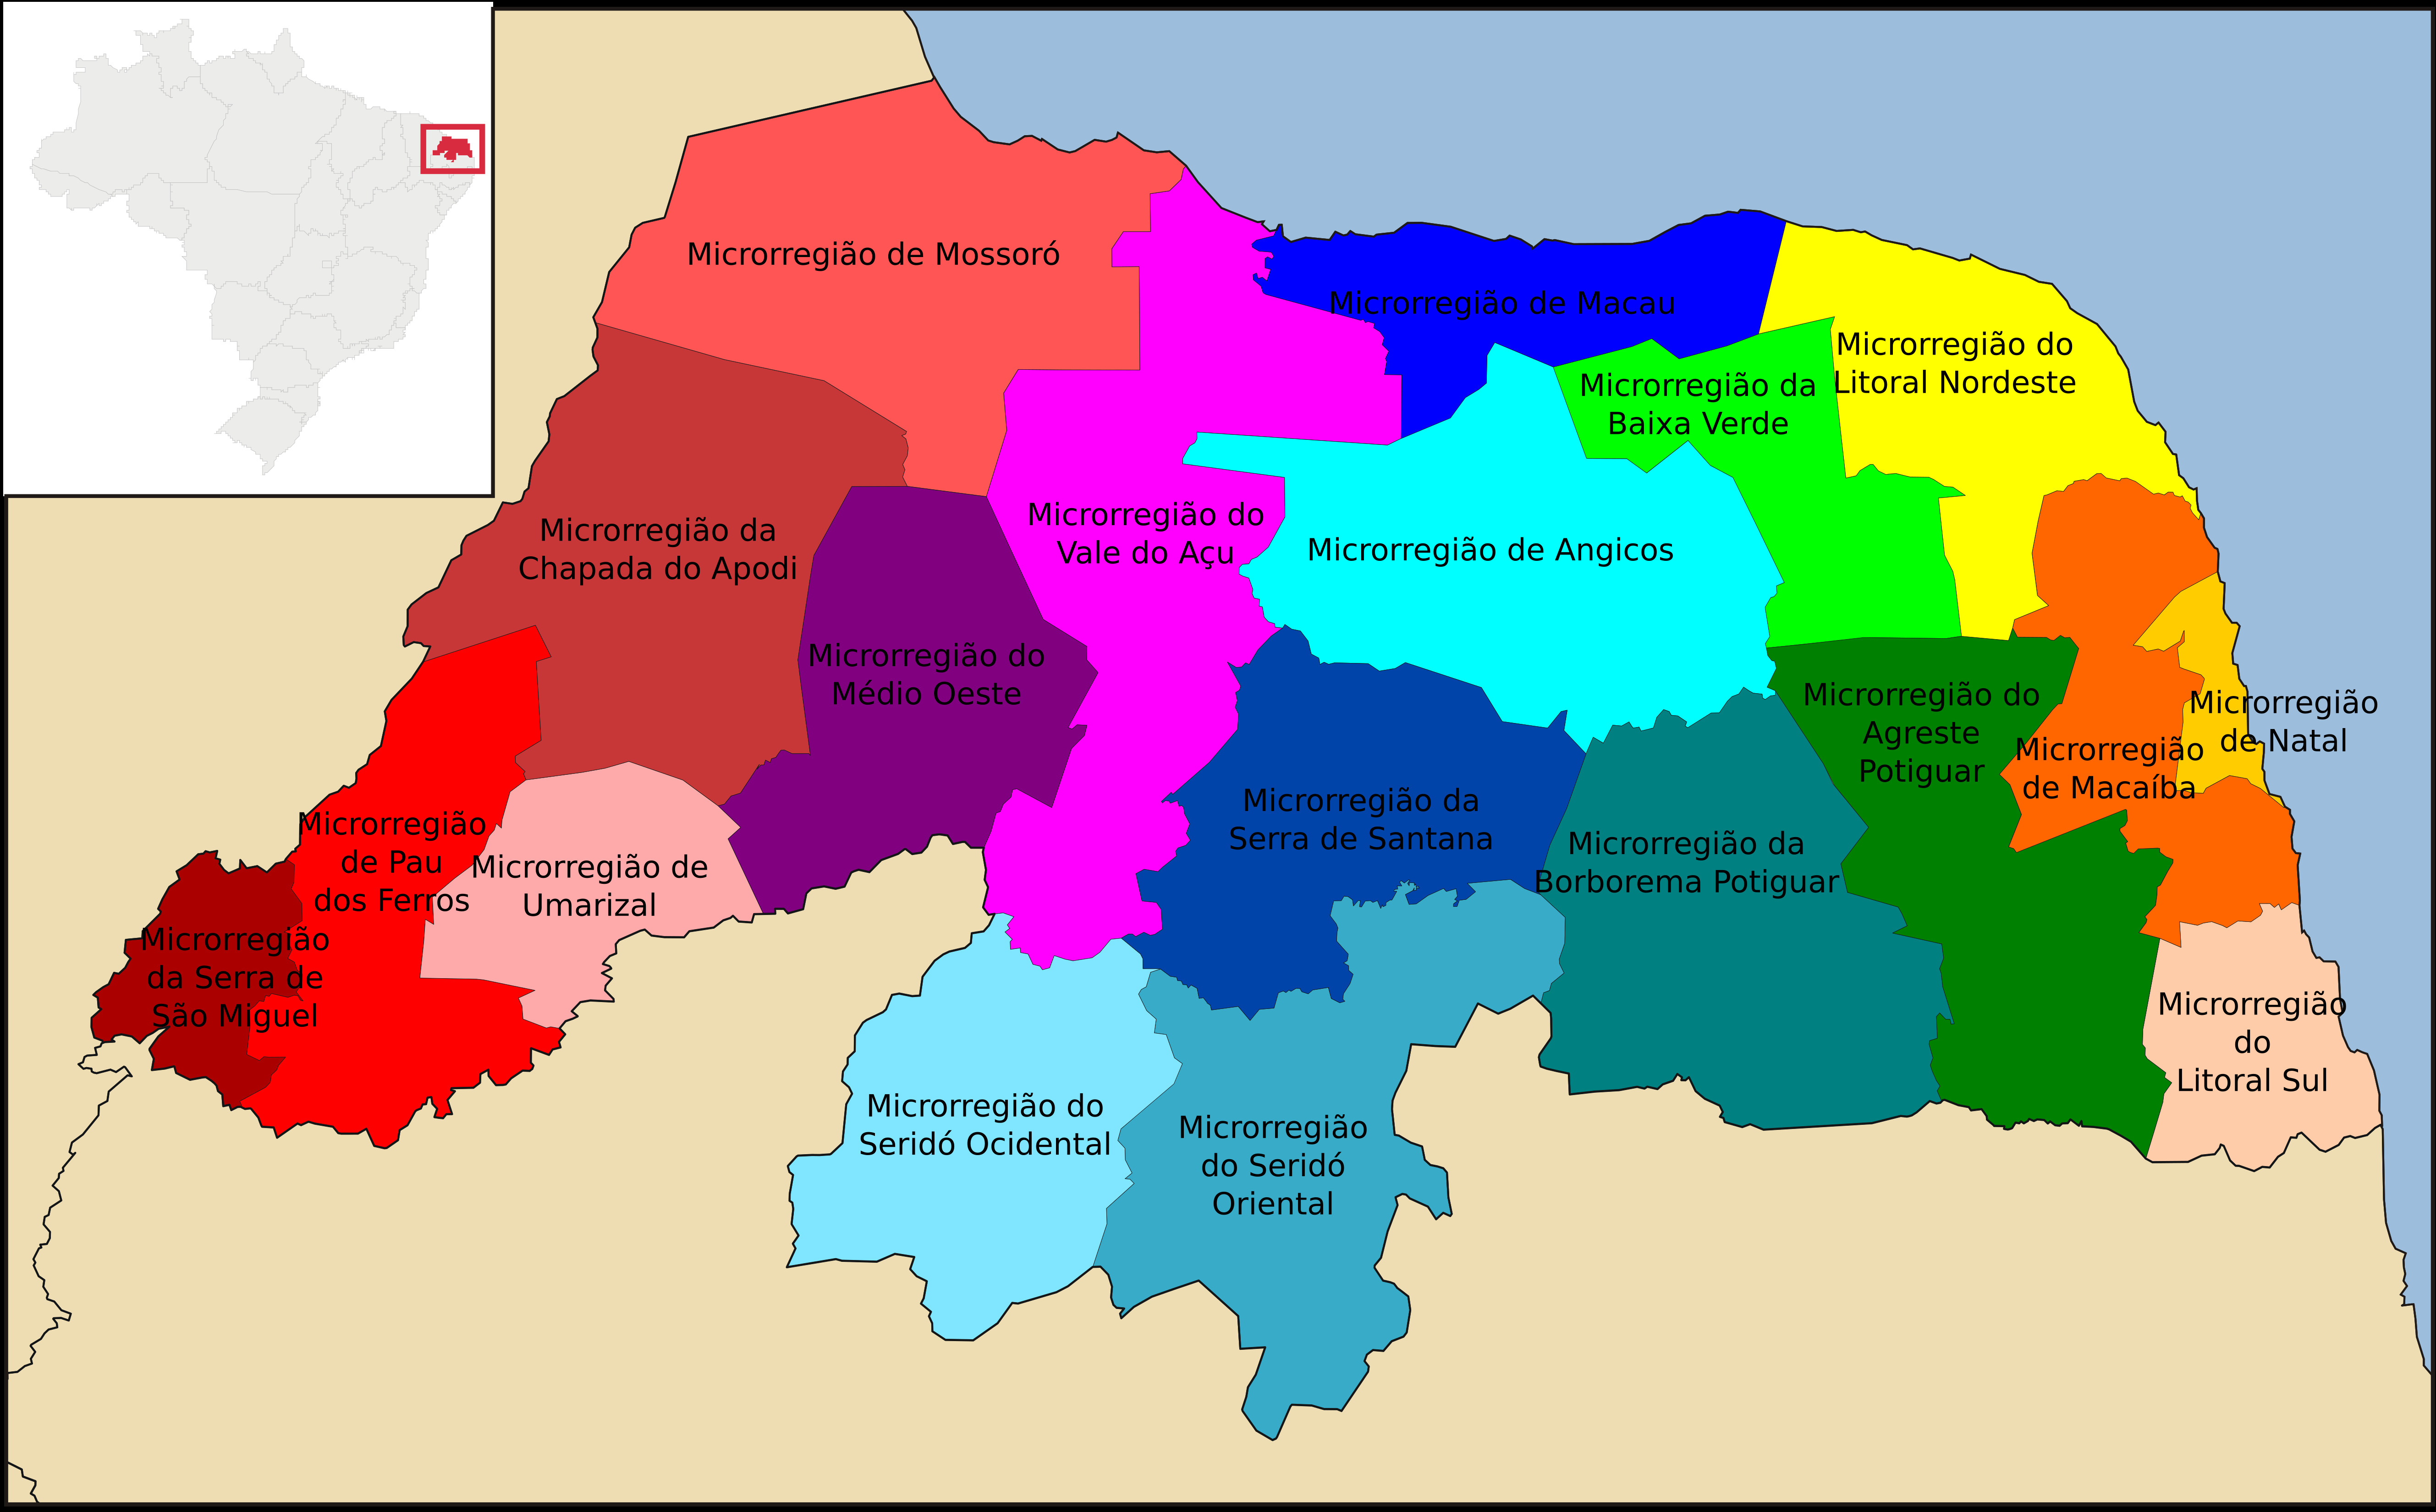
\includegraphics[width=0.8\linewidth]{altoOeste.jpeg}
    \caption{Microrregiões do RN Fonte: \href{https://pt.wikipedia.org/wiki/lista_de_mesorregi\%C3\%B5es_e_microrregi\%C3\%B5es_do_Rio_Grande_do_Norte}{microrregiões do RN}} 
    \label{fig:fig1}
\end{figure}

\section*{Exercício avaliativo:}

Construa um Grafo na qual:

\begin{itemize}
    \item Os \textbf{Vértices} são as cidades.
    \item Se duas cidades são vizinhas, então existe uma \textbf{Aresta} que as conectam.
\end{itemize}

Ver o código exemplo aqui.


Calcule a distância entre todas as cidades listadas nos arquivos {\color{blue} cidades.csv} que tem as localizações definidas por {\color{blue} coordenadas.csv}.

Após calcular 
    

\end{document}